El ancestro común más bajo ({\em Lowest Common Ancestor} (LCA)) es un concepto dentro de la Teoría de grafos y Ciencias de la computación. Sea {\em T} un árbol con raíz y {\em n} nodos. El ancestro común más bajo entre dos nodos {\em v} y {\em w} se define como el nodo más bajo en {\em T} que tiene a {\em v} y {\em w} como descendientes (donde se permite a un nodo ser descendiente de él mismo).

\begin{figure}[!h]
	\centering
	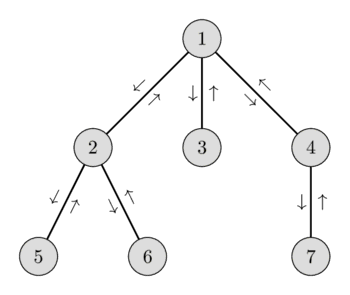
\includegraphics[width=0.35\linewidth]{img/LCA_Euler}

	\label{fig:lcaeuler}
\end{figure} 

Para el caso de la imagen anterior el $LCA(5,6)=2$ , $LCA(3,6)=1$ y $LCA(2,6)=2$.